Referred to \cite{CMS-PAS-HIG-19-001}.
%
%Similar to electrons the muon momentum scale is measured in data by fitting a Crystall-ball function to the di-muon mass spectrum around the Z peak in the 
%$Z \rightarrow \mu\mu$ control region. %At the moment no muon scale and resolution corrections are available but from 
%Fig.~\ref{fig:mu_energy_scaleA},~\ref{fig:mu_energy_scaleB} and~\ref{fig:mu_energy_scaleC} shows a very good agreement between data and simulation, for 2016, 2017 and 2018 eras, respectively. %even without any corrections.
%
%\begin{figure}[!htb]
%	\vspace*{0.3cm}
%	\begin{center}
%		\subfigure [] {\resizebox{8cm}{!}{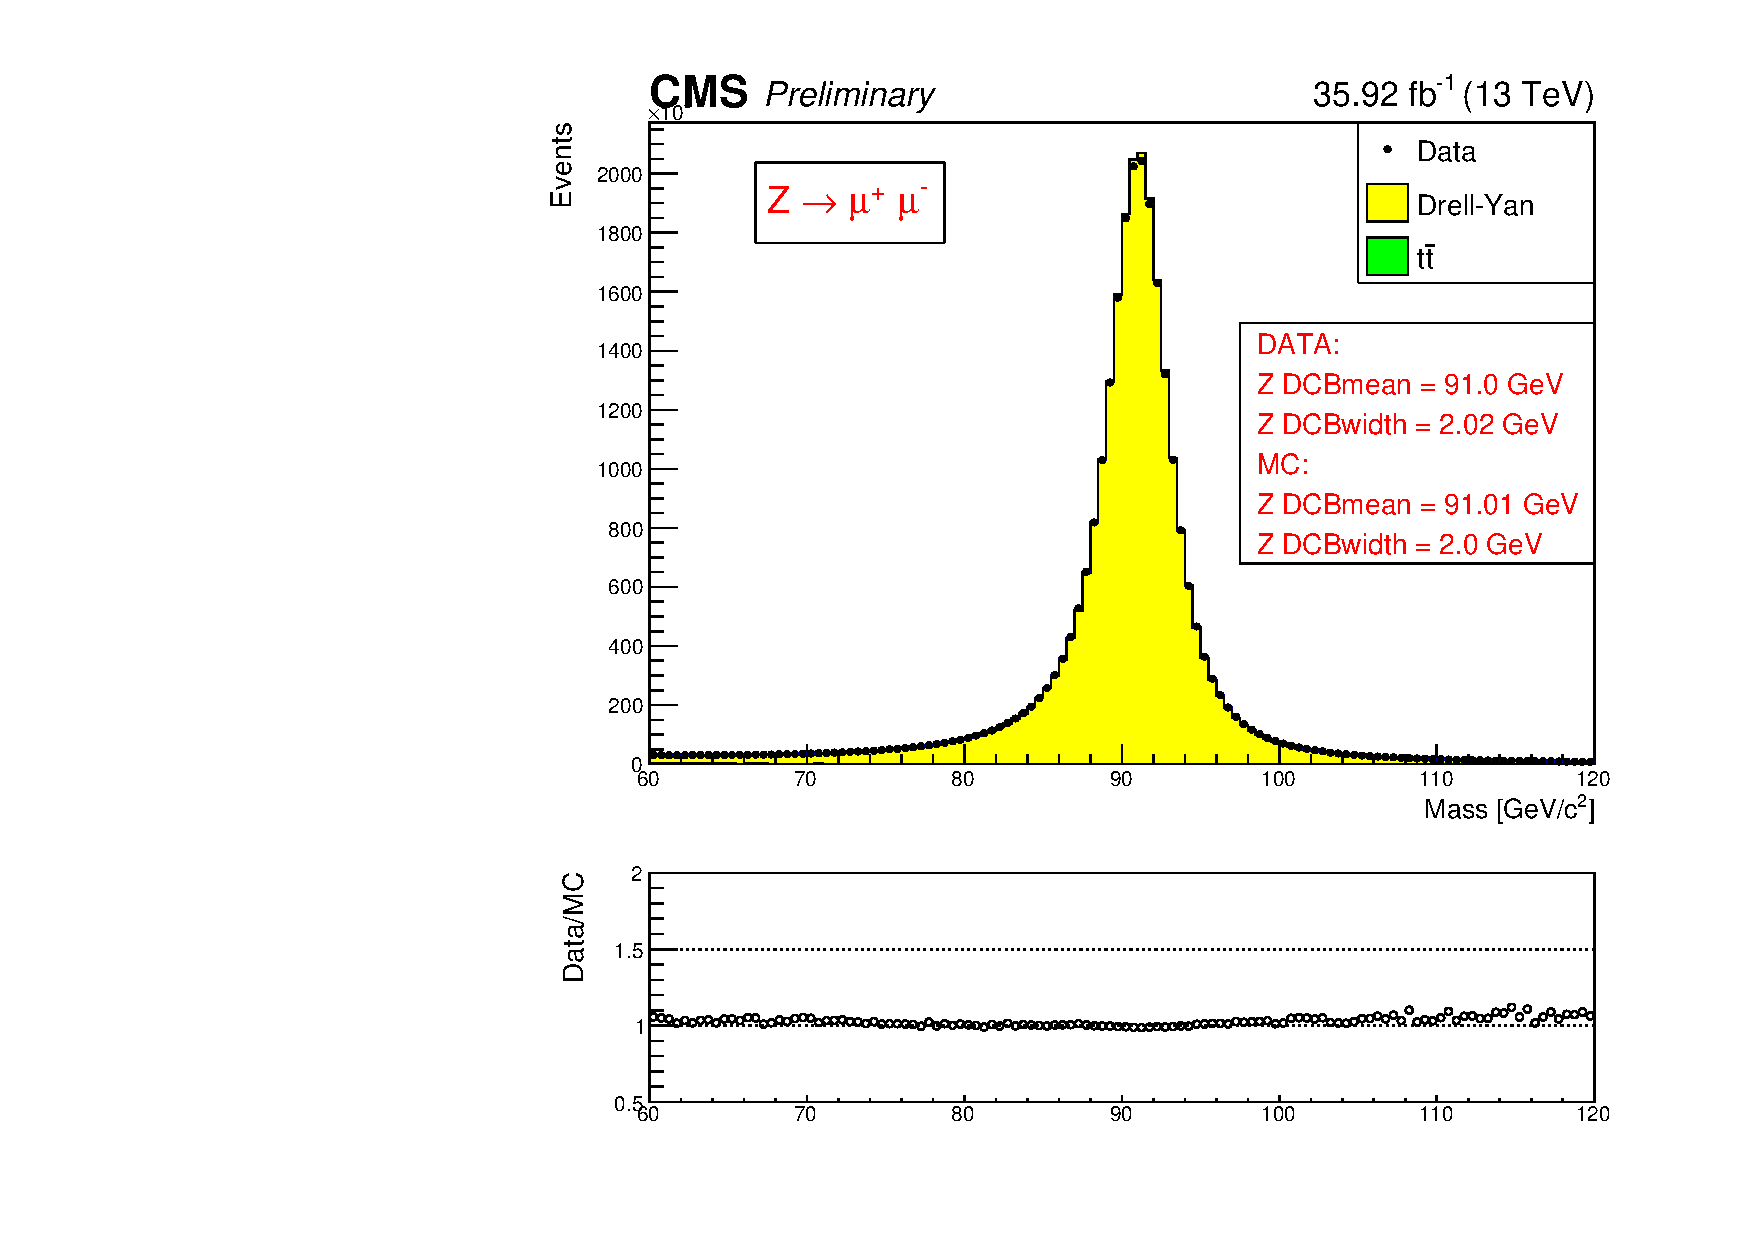
\includegraphics{Figures/Muons/2016_ZMass_mu.pdf}}}
%		\subfigure [] {\resizebox{8cm}{!}{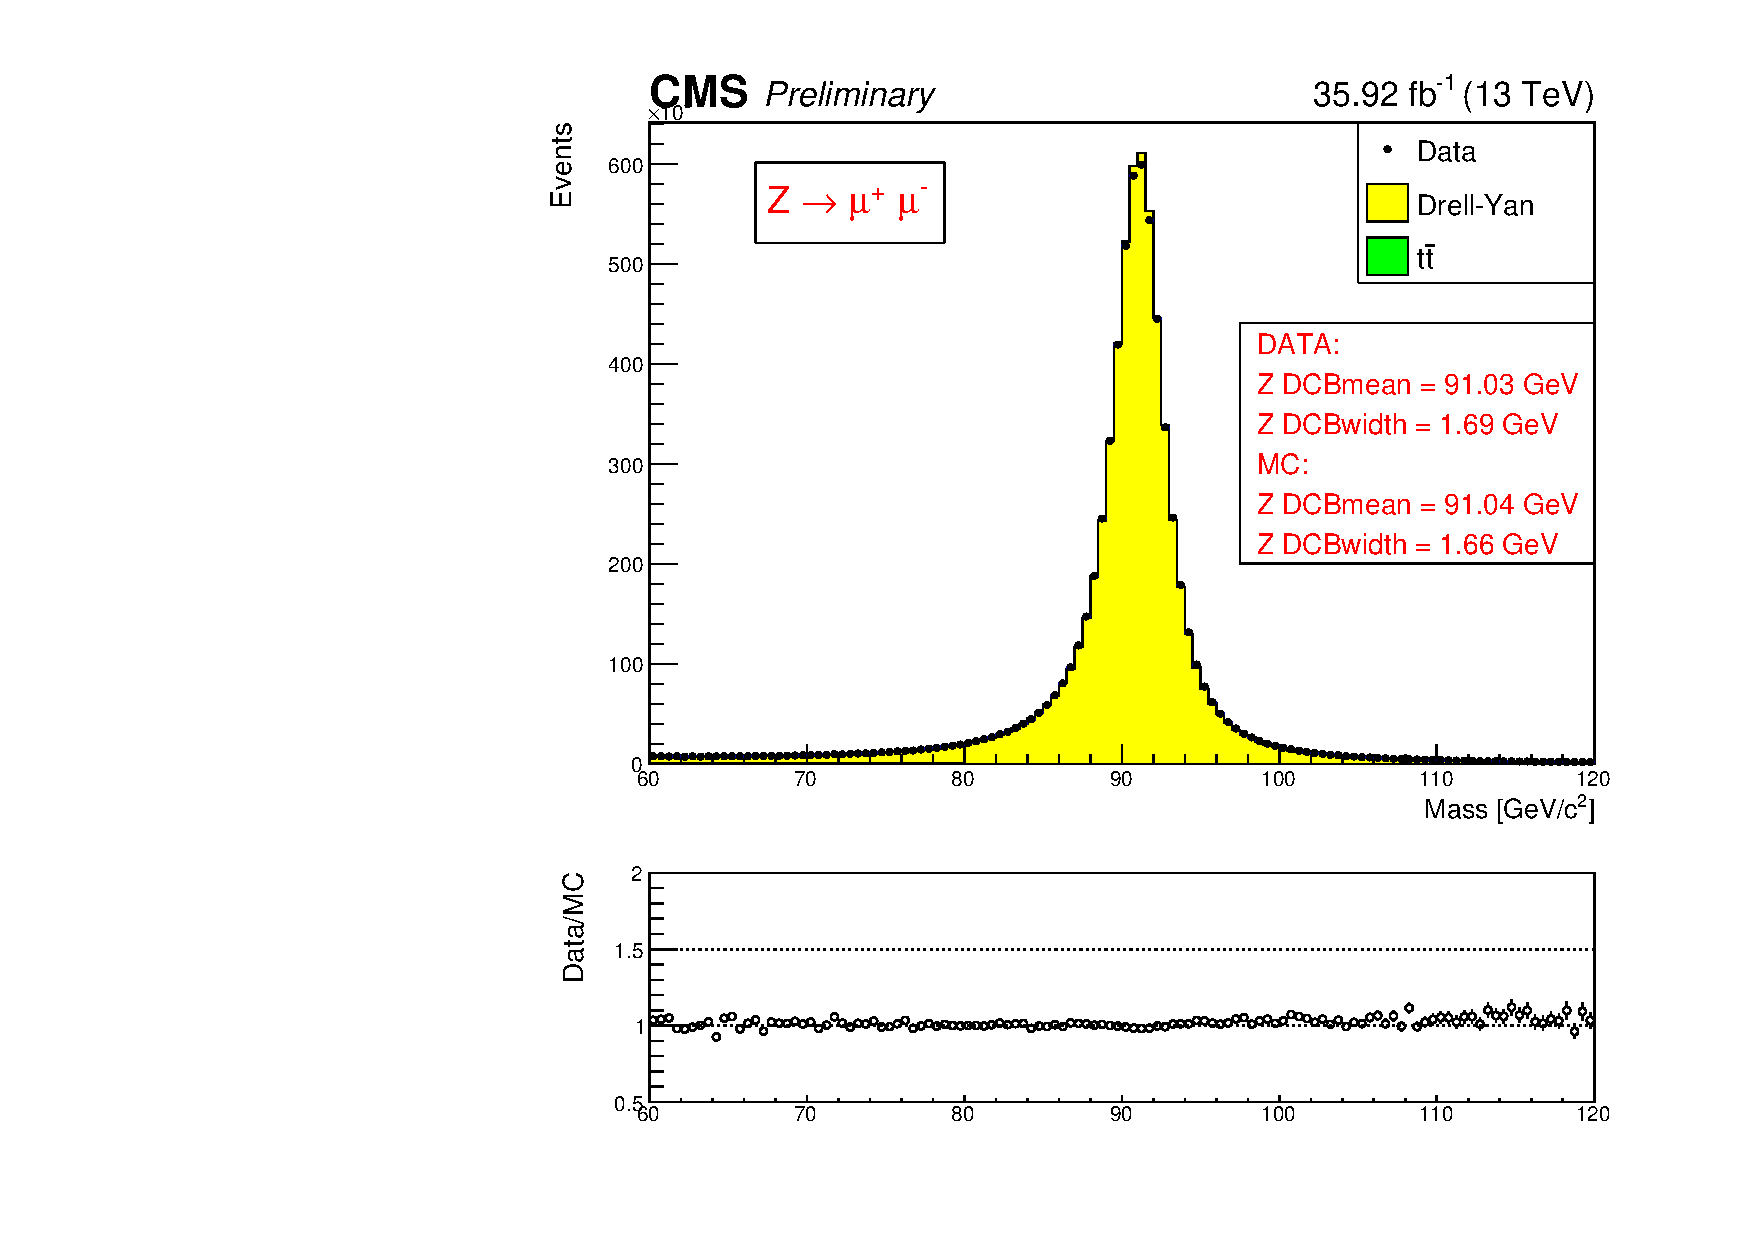
\includegraphics{Figures/Muons/2016_ZMass_mu_MBMB.pdf}}} \\
%		\subfigure [] {\resizebox{8cm}{!}{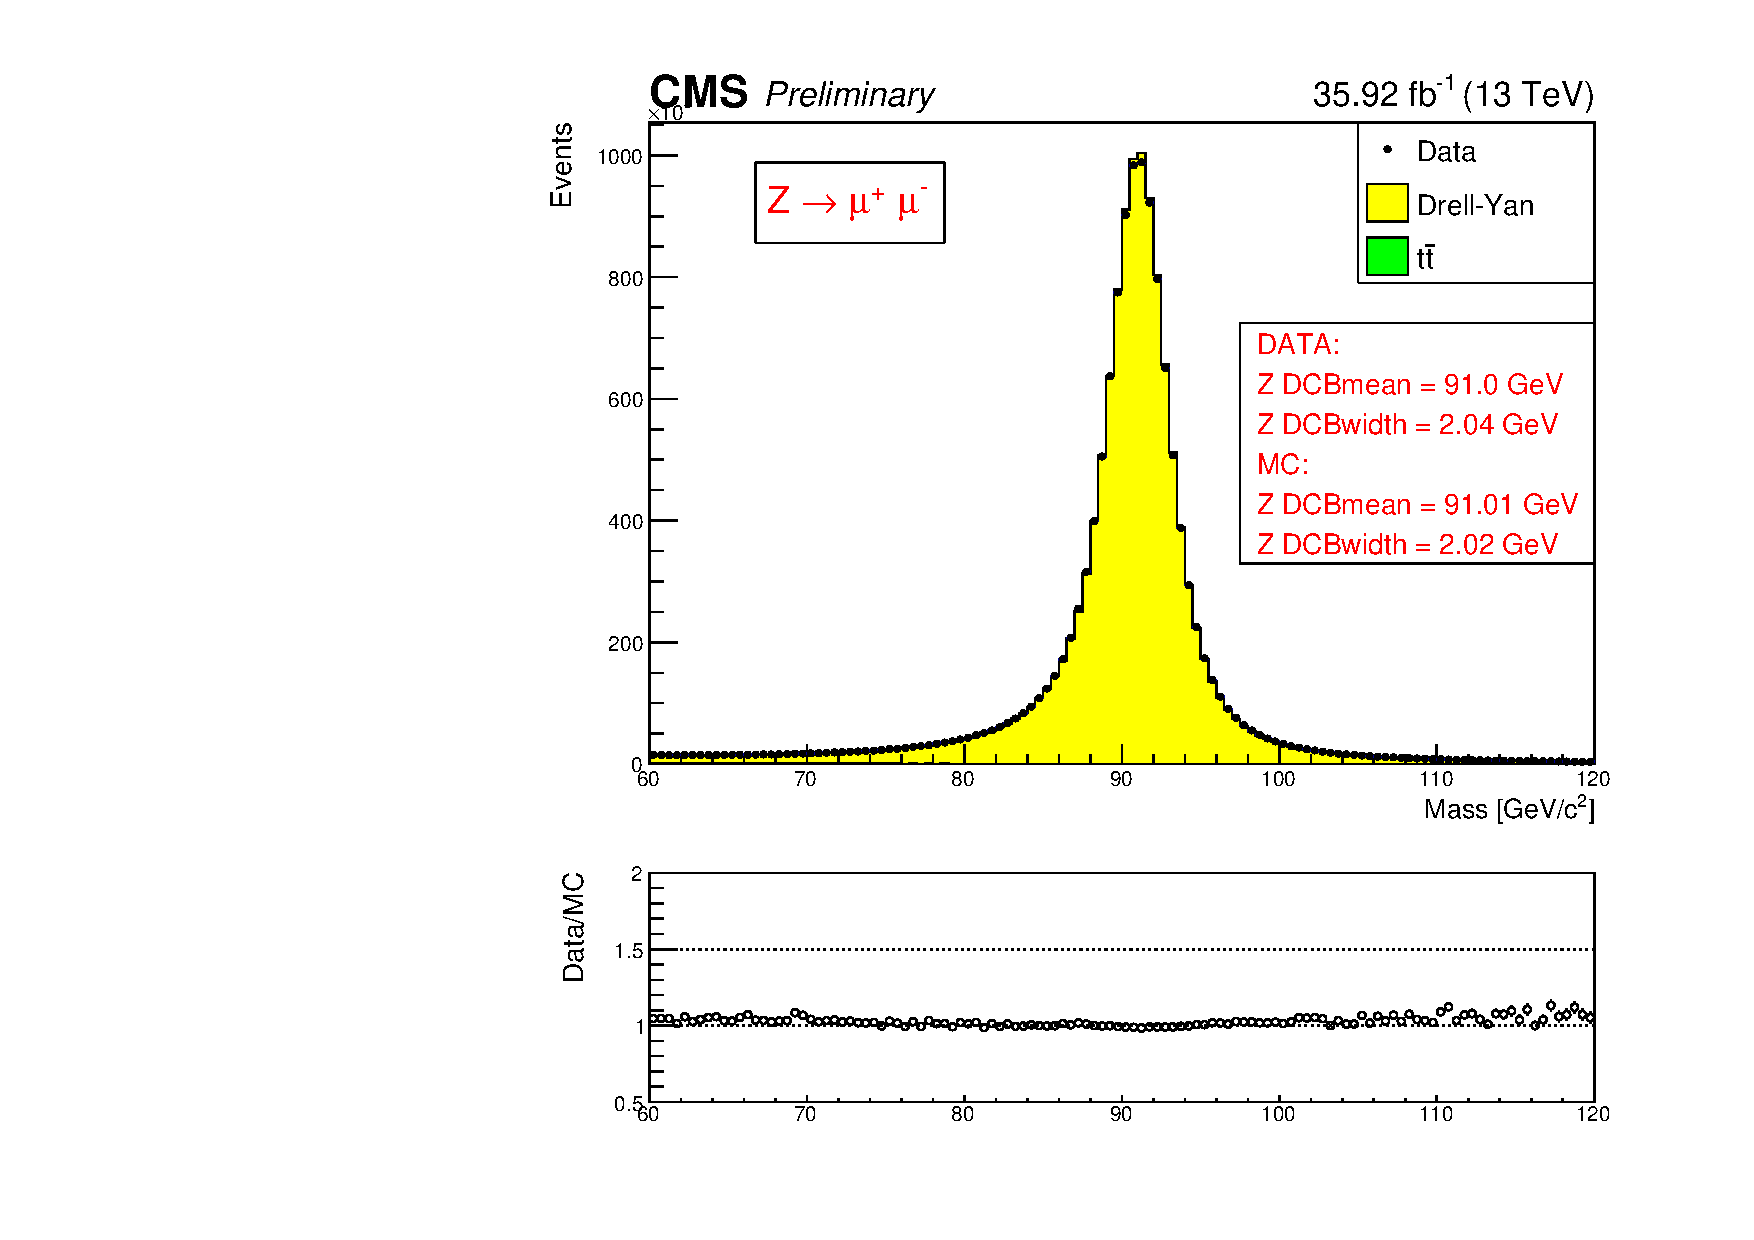
\includegraphics{Figures/Muons/2016_ZMass_mu_MBME.pdf}}}
%		\subfigure [] {\resizebox{8cm}{!}{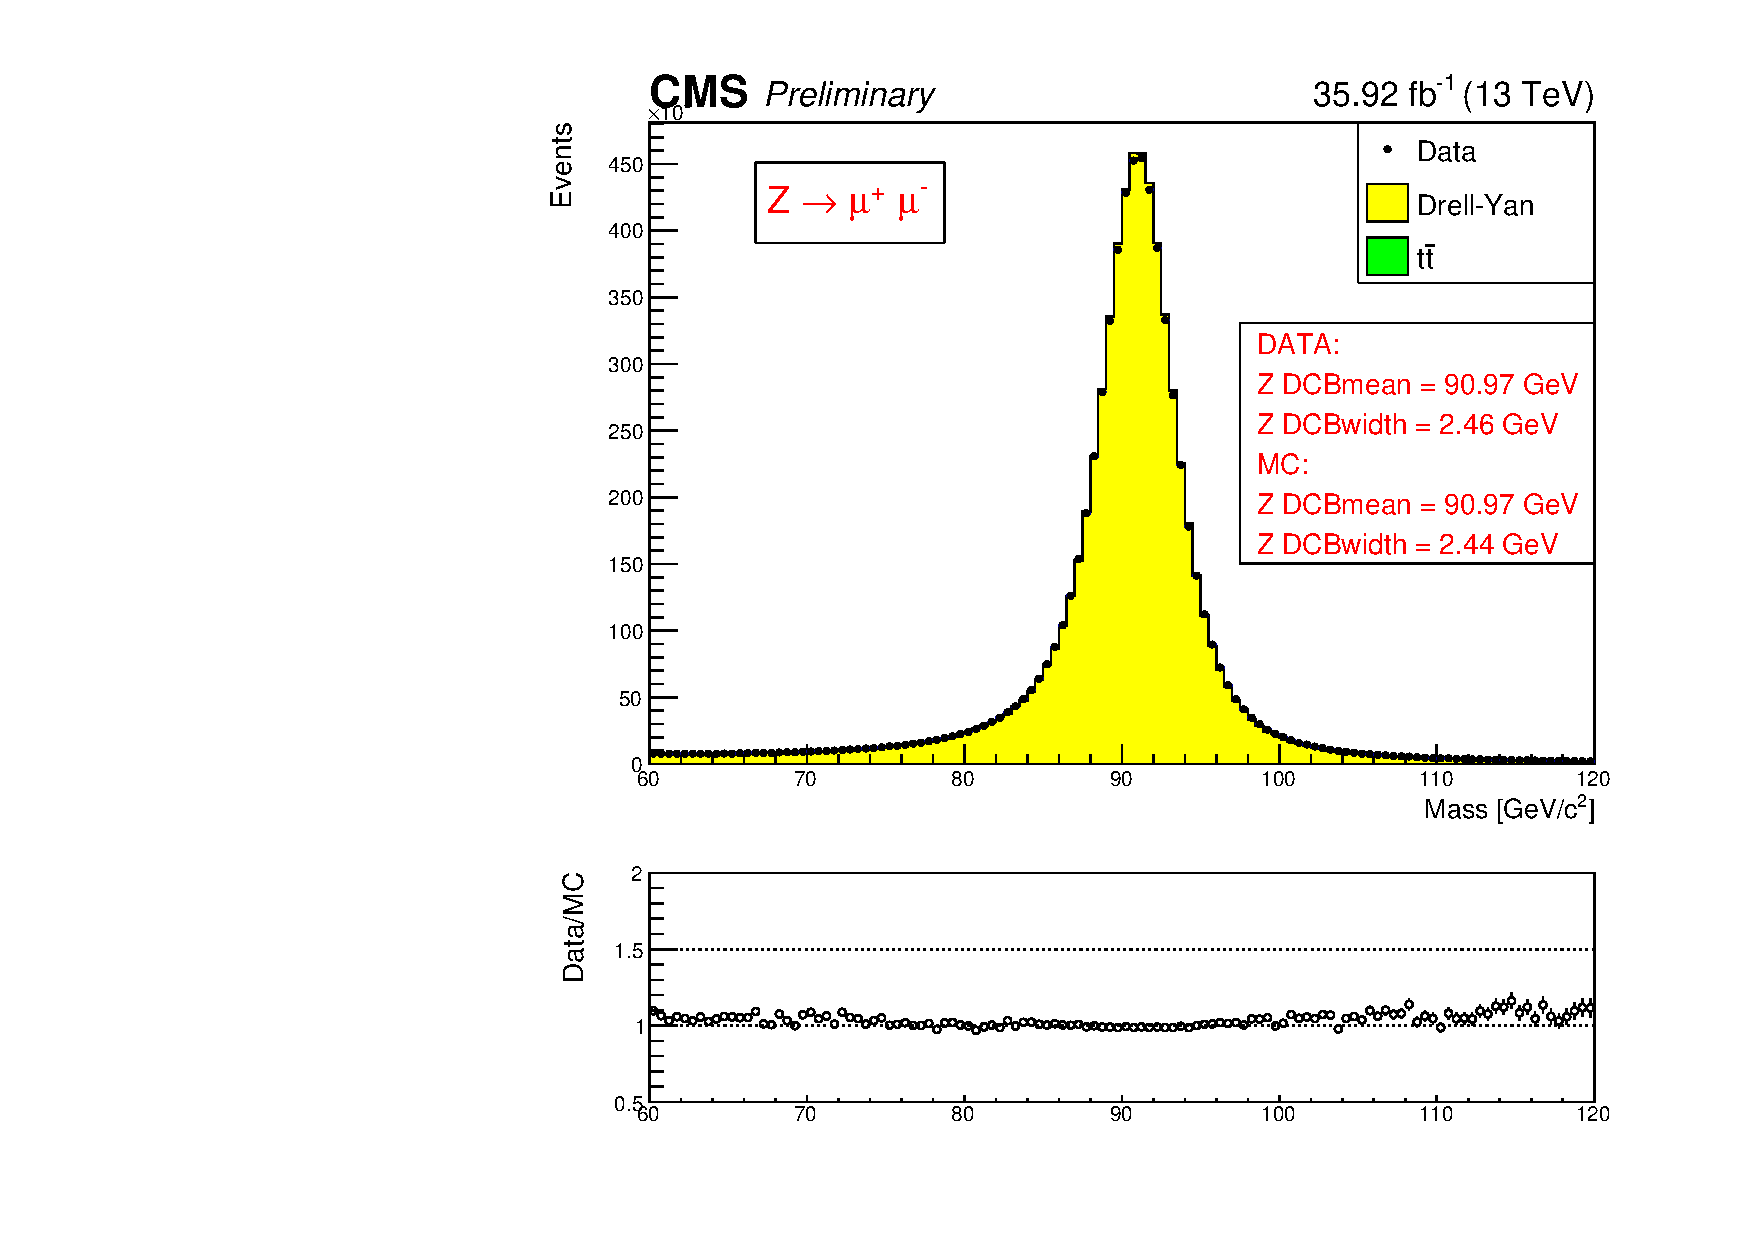
\includegraphics{Figures/Muons/2016_ZMass_mu_MEME.pdf}}} \\
%	\end{center}
%	\caption{
%		(a): muon energy scale measured in the $Z\rightarrow \mu \mu$ control region for all muons, for both muons in the barrel (b), for one muon in the barrel, one in the endcaps (c) and for both muons in the endcaps (d), for 2016.
%		The results of the Crystall-ball fit are reported in the figures.
%		%\textbf{FIXME: mu-scale and smearing corrections NOT yet available and thus NOT yet applied} 
%	}
%	\label{fig:mu_energy_scaleA}
%\end{figure}
%
%\begin{figure}[!htb]
%	\vspace*{0.3cm}
%	\begin{center}
%		\subfigure [] {\resizebox{8cm}{!}{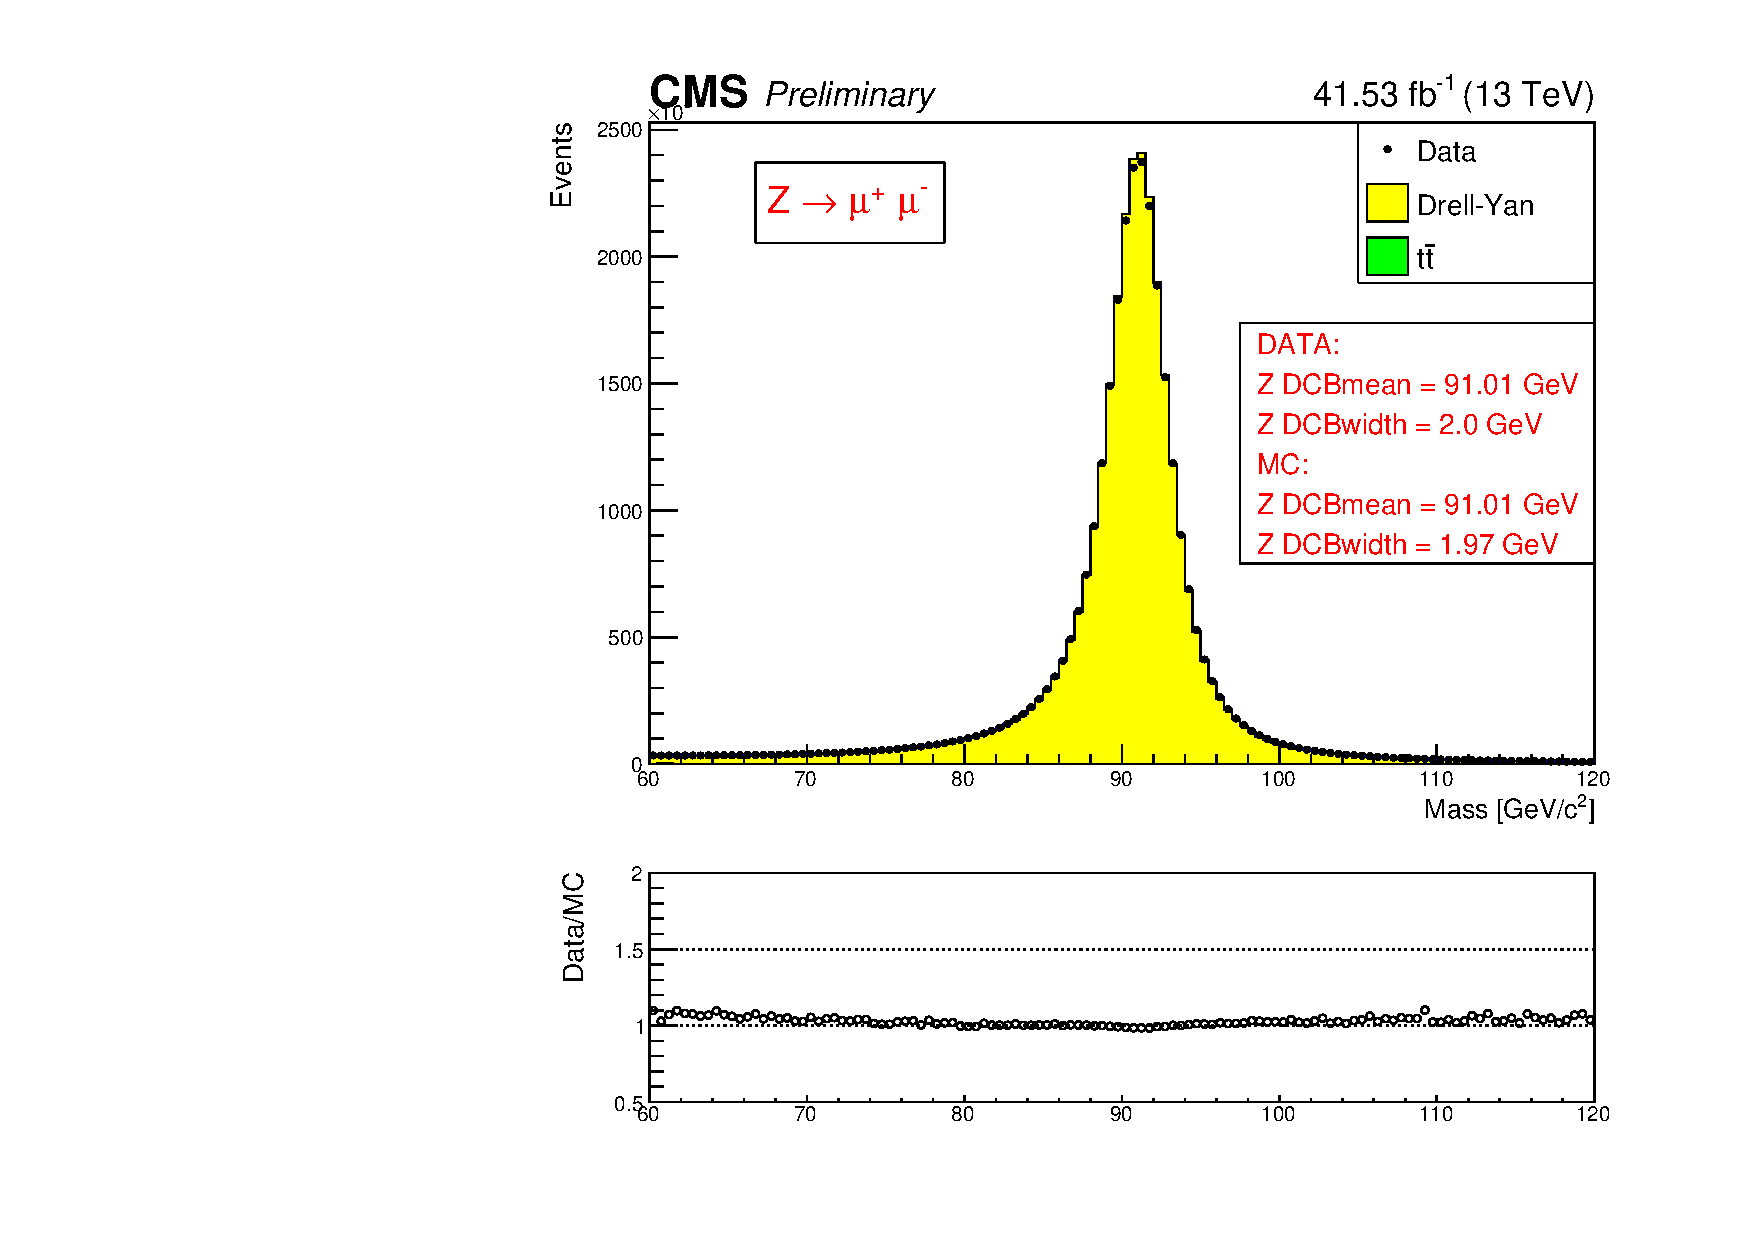
\includegraphics{Figures/Muons/2017_ZMass_mu.pdf}}}
%		\subfigure [] {\resizebox{8cm}{!}{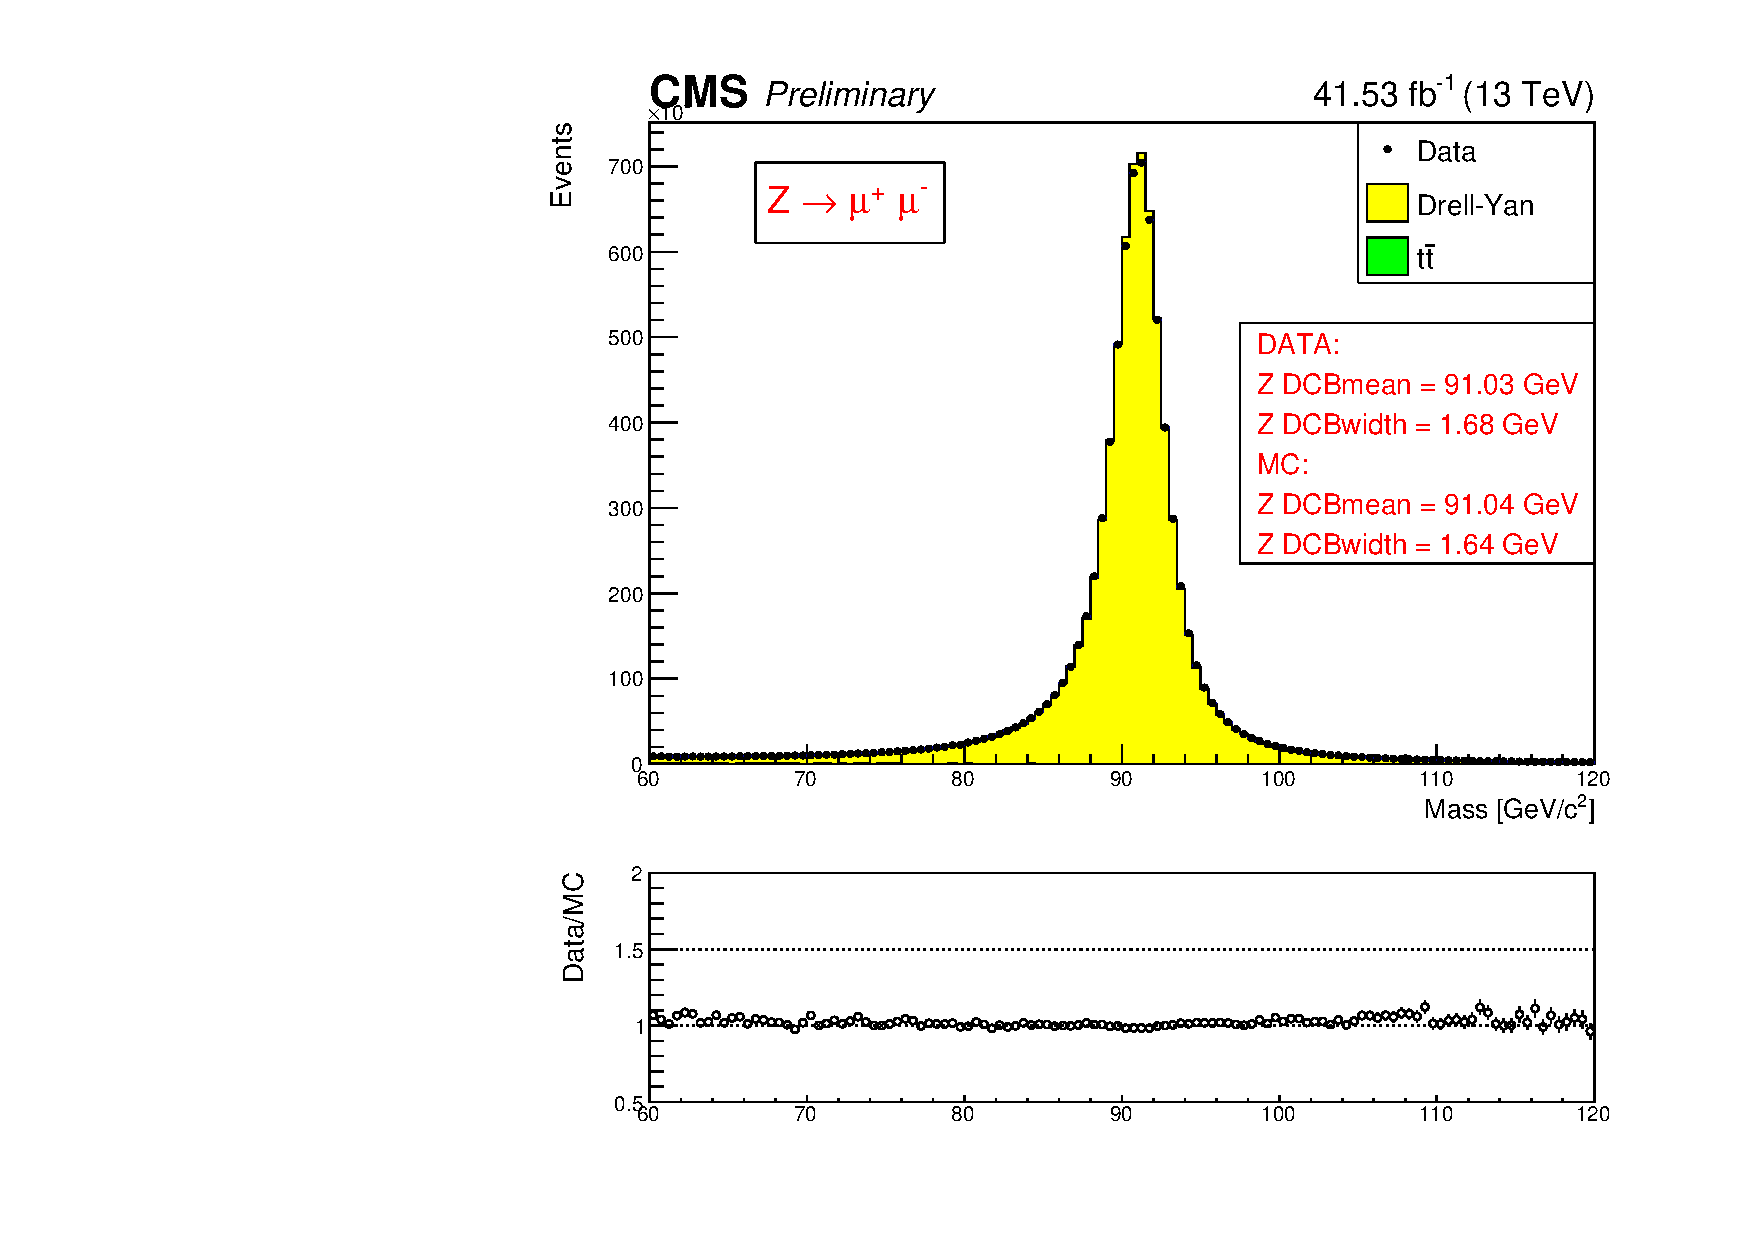
\includegraphics{Figures/Muons/2017_ZMass_mu_MBMB.pdf}}} \\
%		\subfigure [] {\resizebox{8cm}{!}{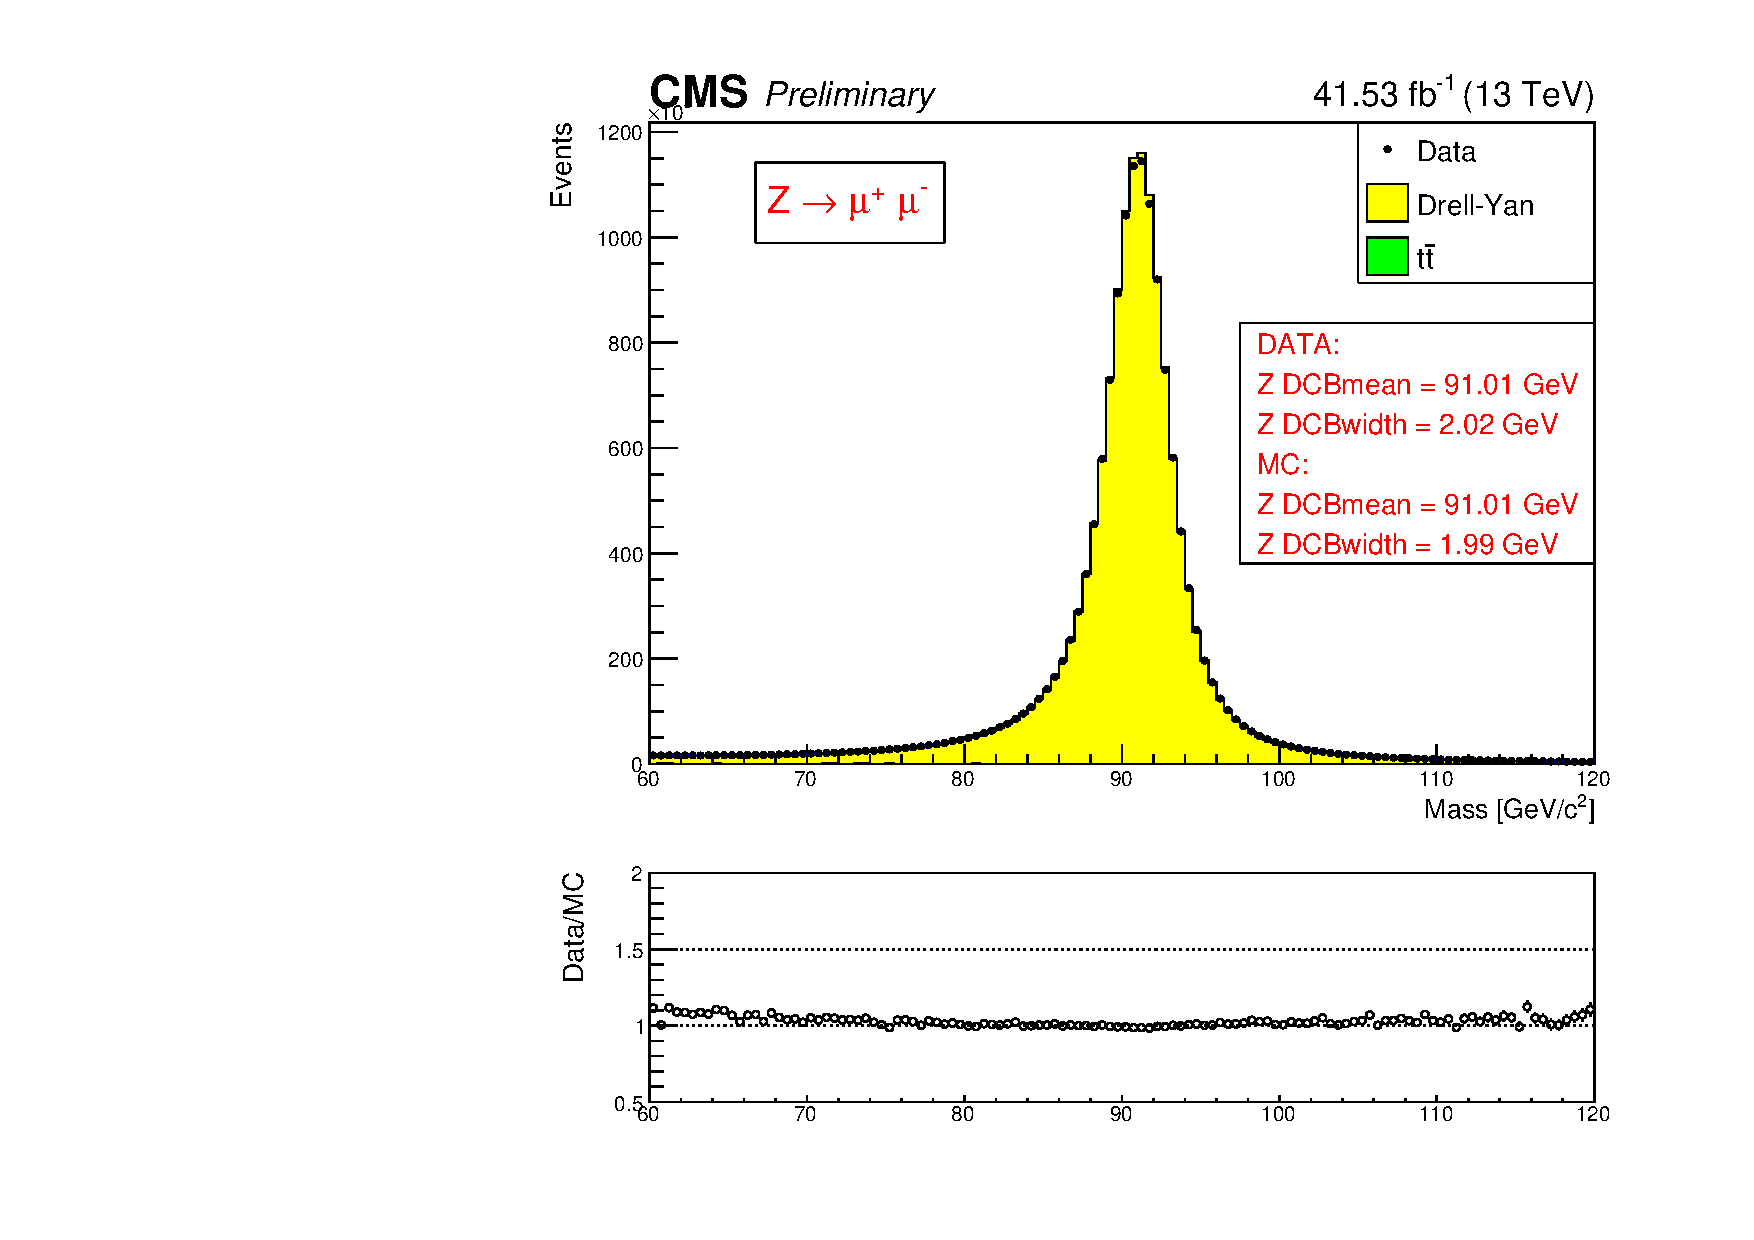
\includegraphics{Figures/Muons/2017_ZMass_mu_MBME.pdf}}}
%		\subfigure [] {\resizebox{8cm}{!}{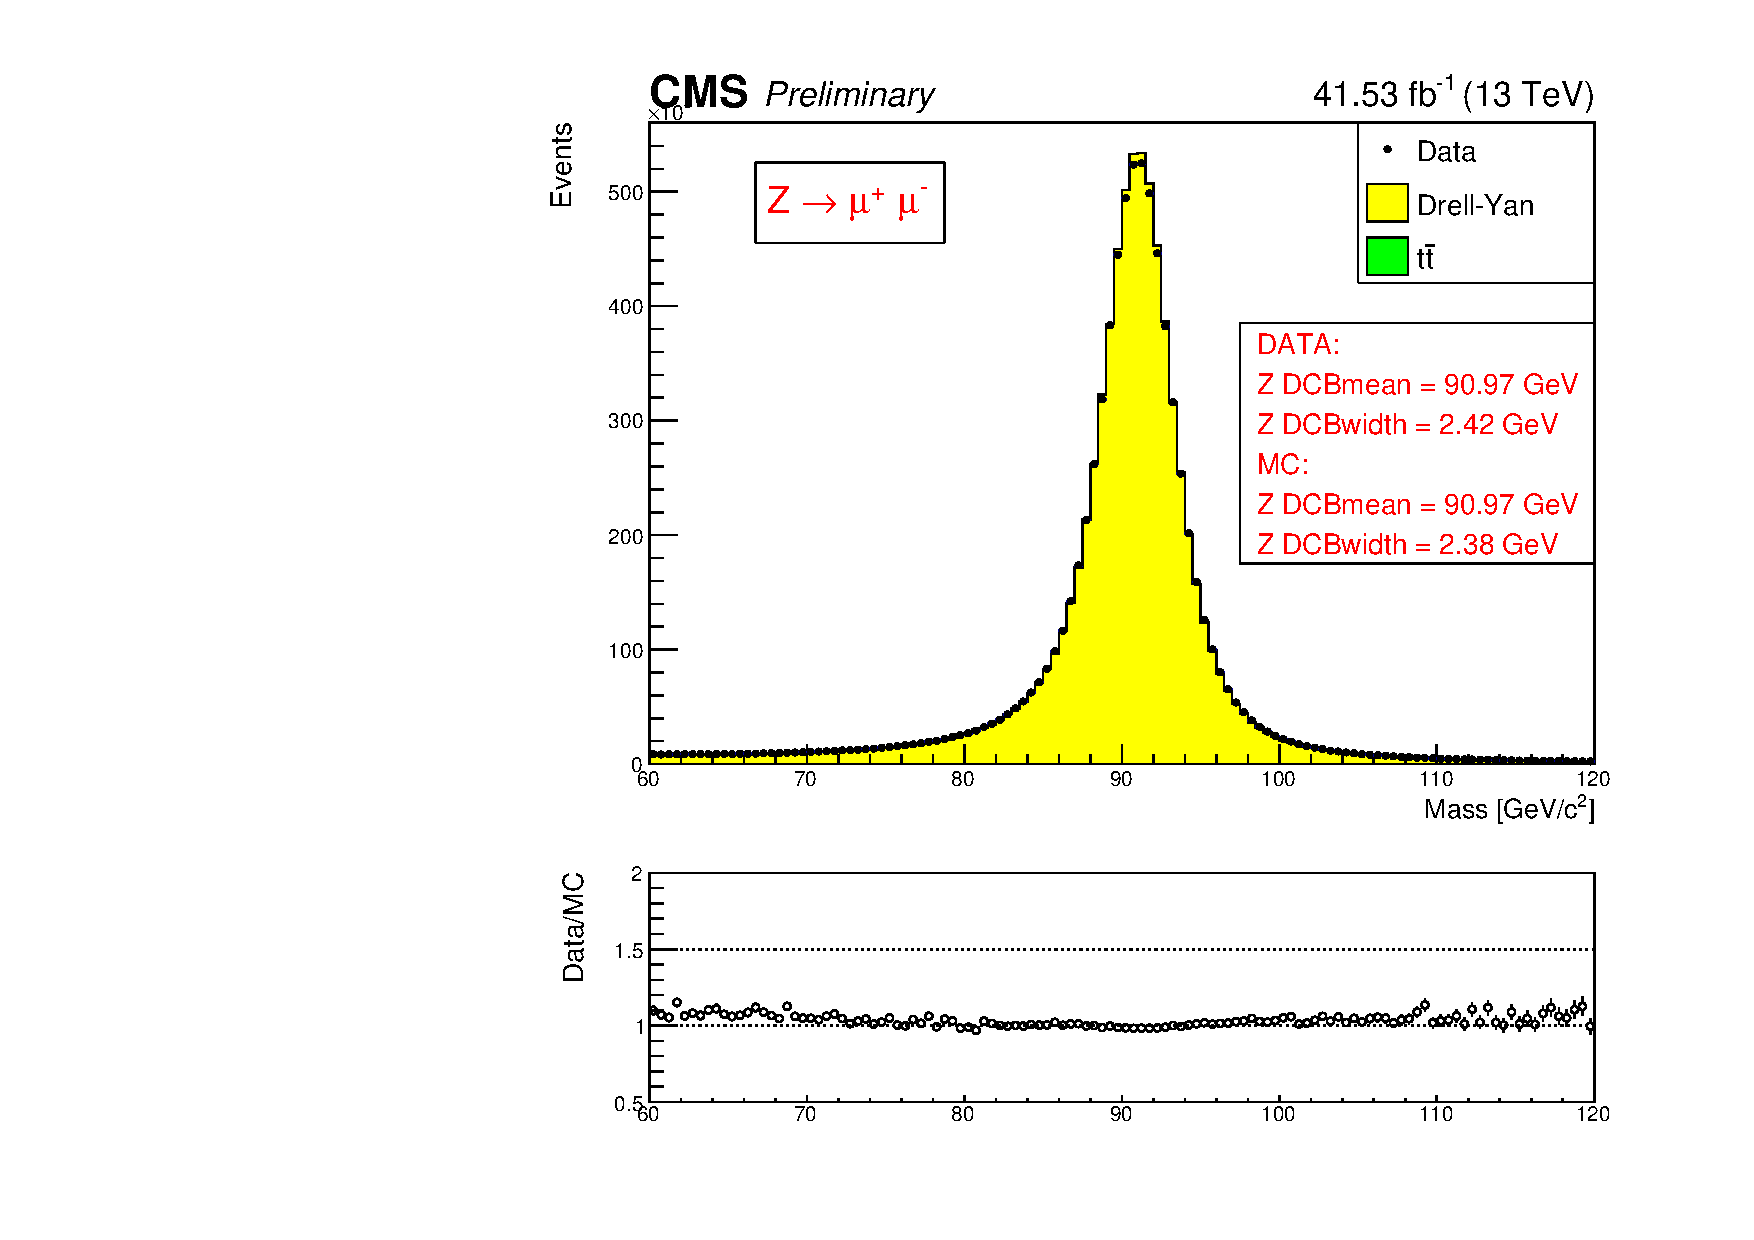
\includegraphics{Figures/Muons/2017_ZMass_mu_MEME.pdf}}} \\
%	\end{center}
%	\caption{
%		(a): muon energy scale measured in the $Z\rightarrow \mu \mu$ control region for all muons, for both muons in the barrel (b), for one muon in the barrel, one in the endcaps (c) and for both muons in the endcaps (d), for 2017.
%		The results of the Crystall-ball fit are reported in the figures.
%		%\textbf{FIXME: mu-scale and smearing corrections NOT yet available and thus NOT yet applied} 
%	}
%	\label{fig:mu_energy_scaleB}
%\end{figure}
%
%
%\begin{figure}[!htb]
%	\vspace*{0.3cm}
%	\begin{center}
%		\subfigure [] {\resizebox{8cm}{!}{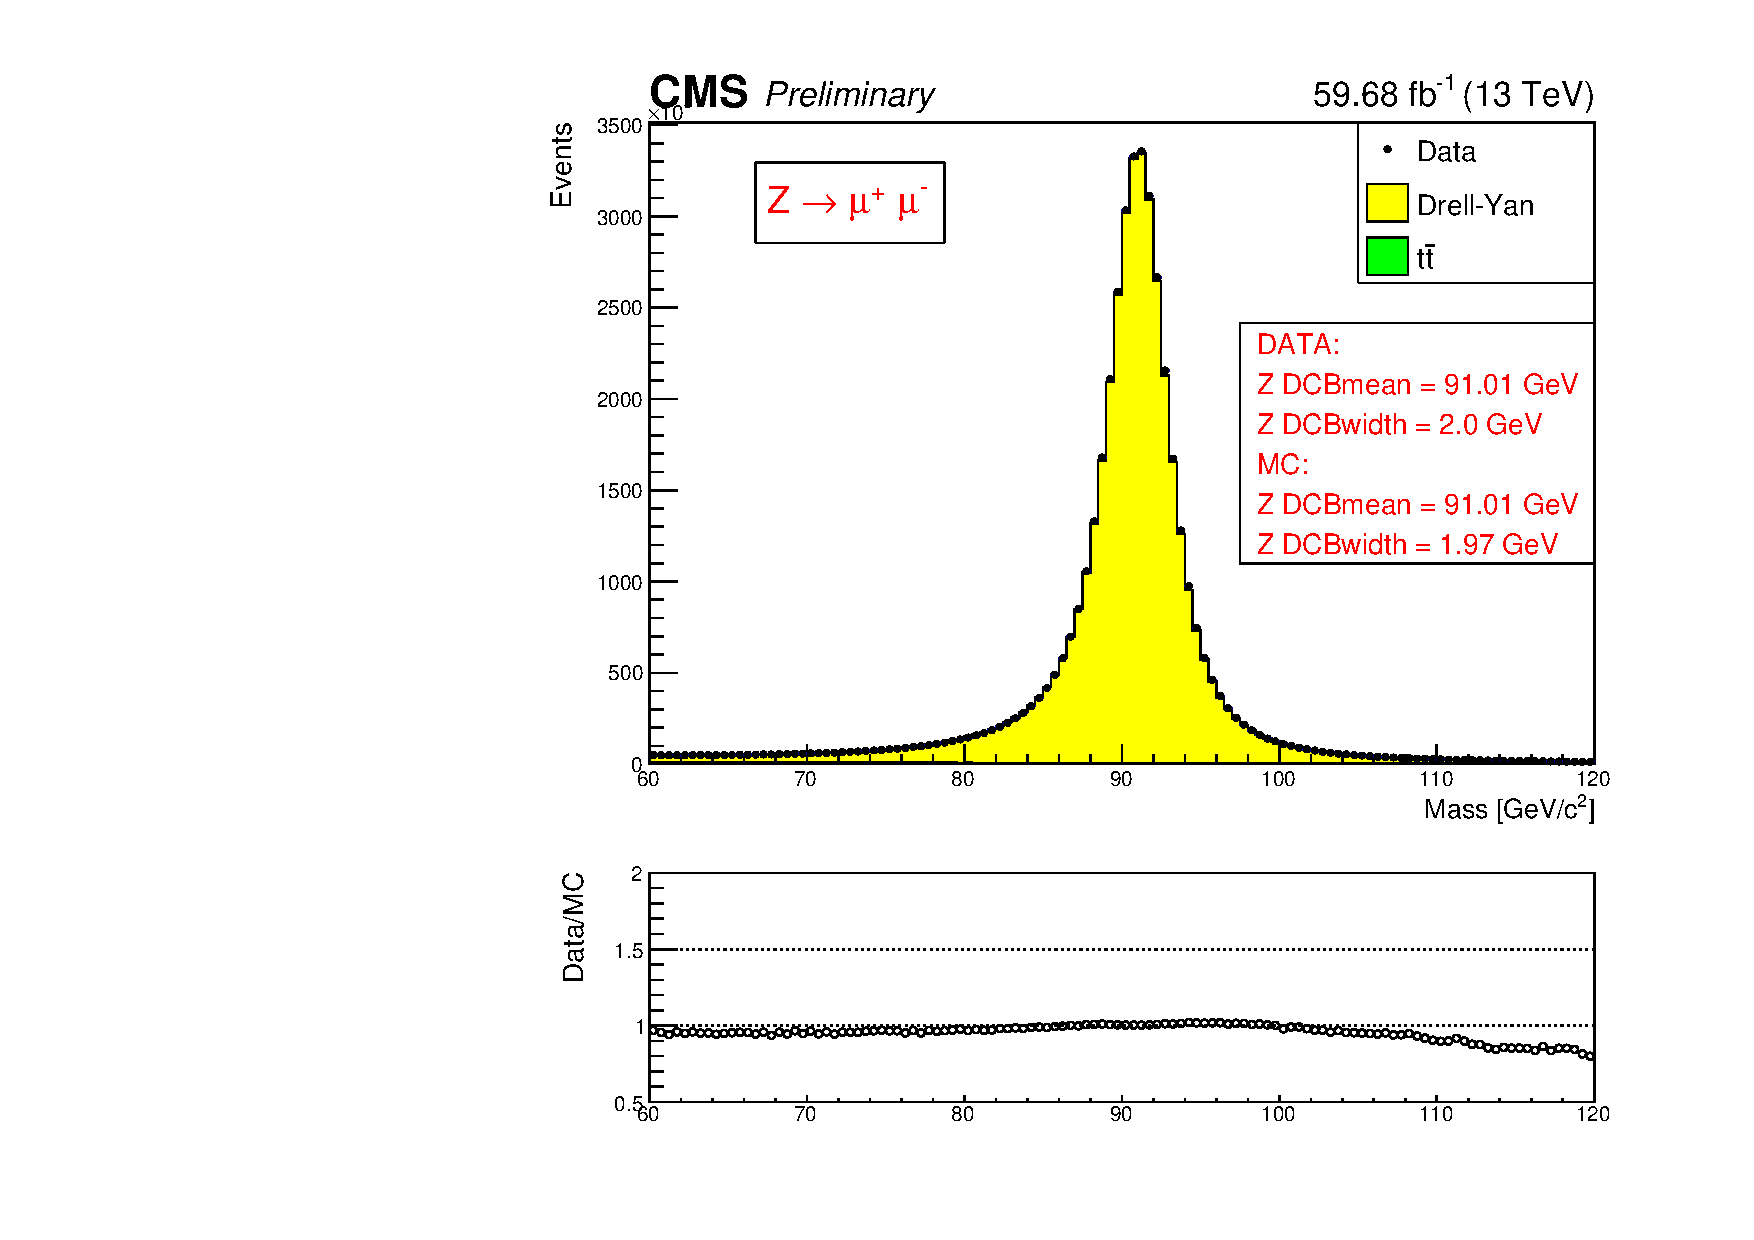
\includegraphics{Figures/Muons/2018_ZMass_mu.pdf}}}
%		\subfigure [] {\resizebox{8cm}{!}{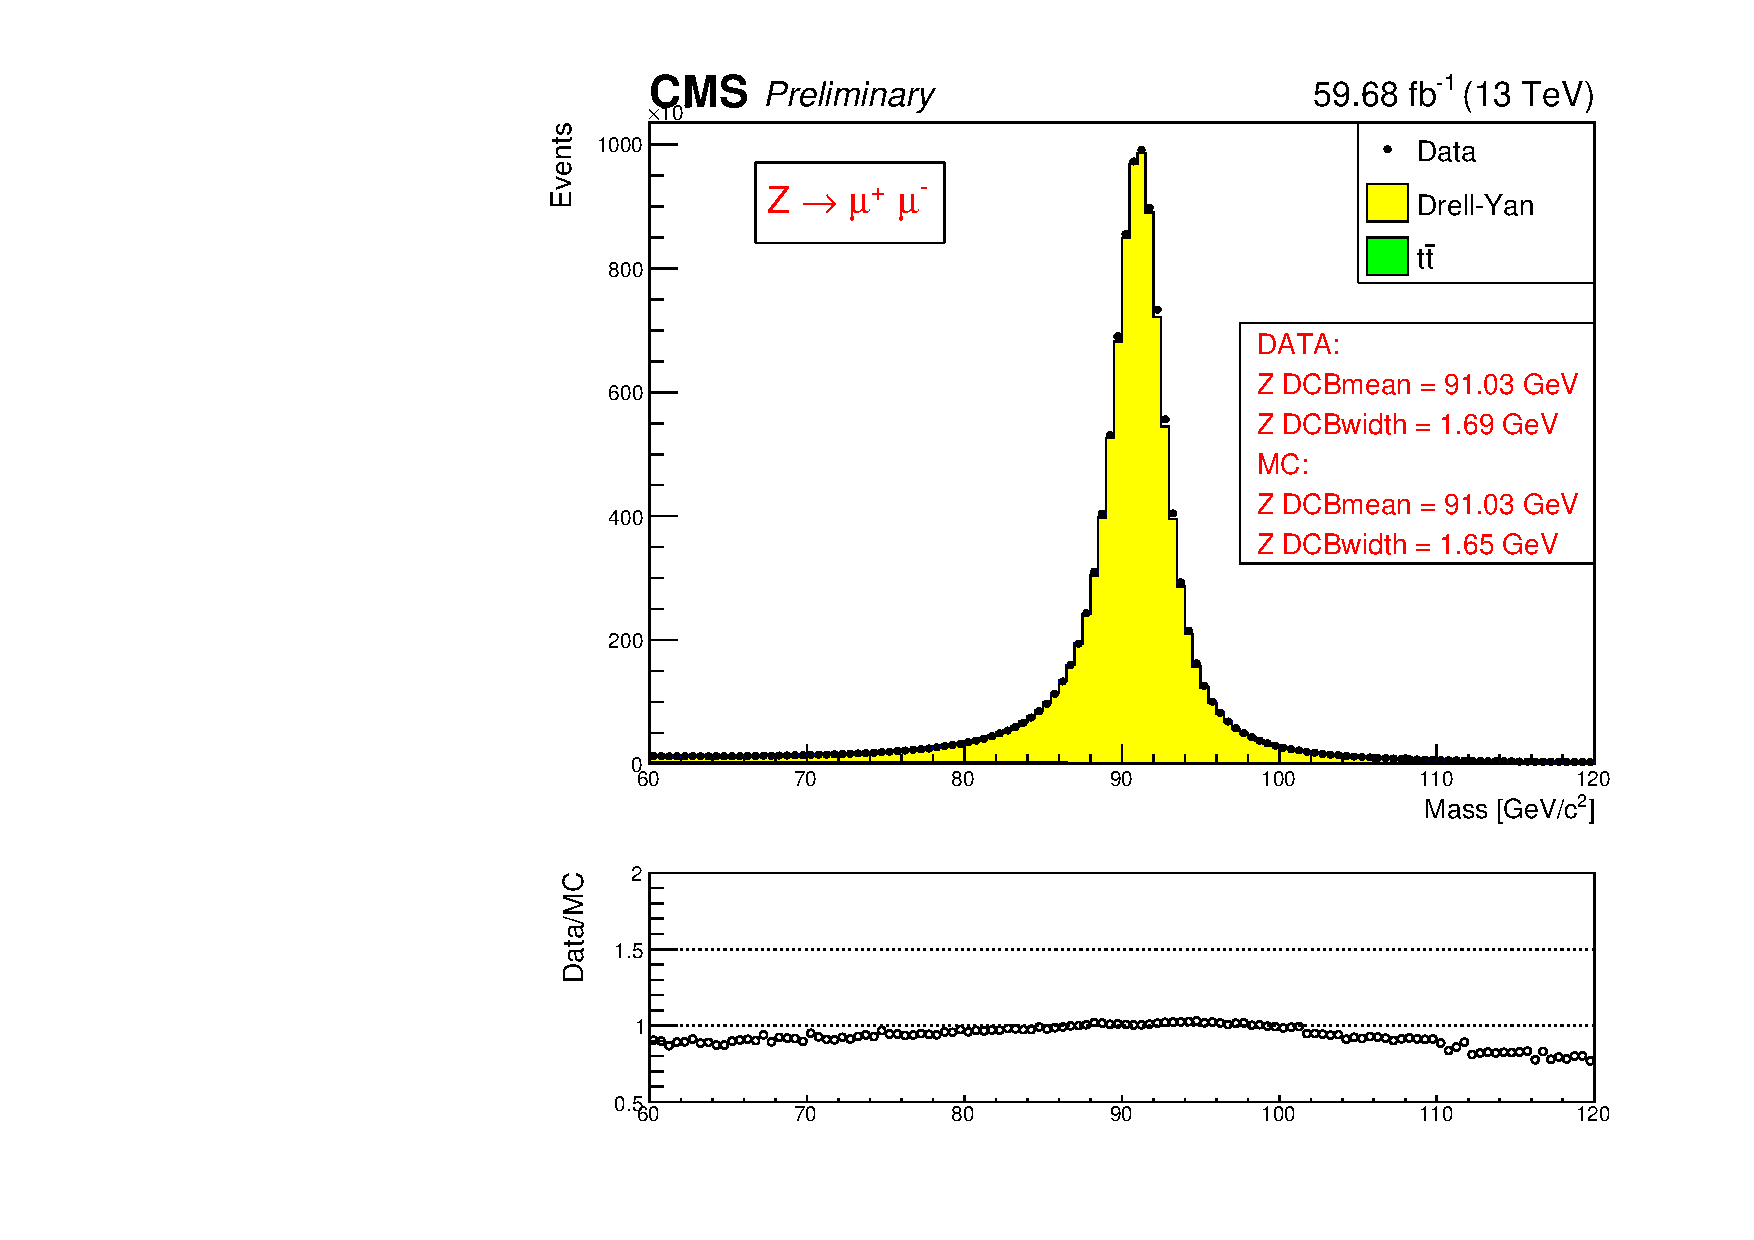
\includegraphics{Figures/Muons/2018_ZMass_mu_MBMB.pdf}}} \\
%		\subfigure [] {\resizebox{8cm}{!}{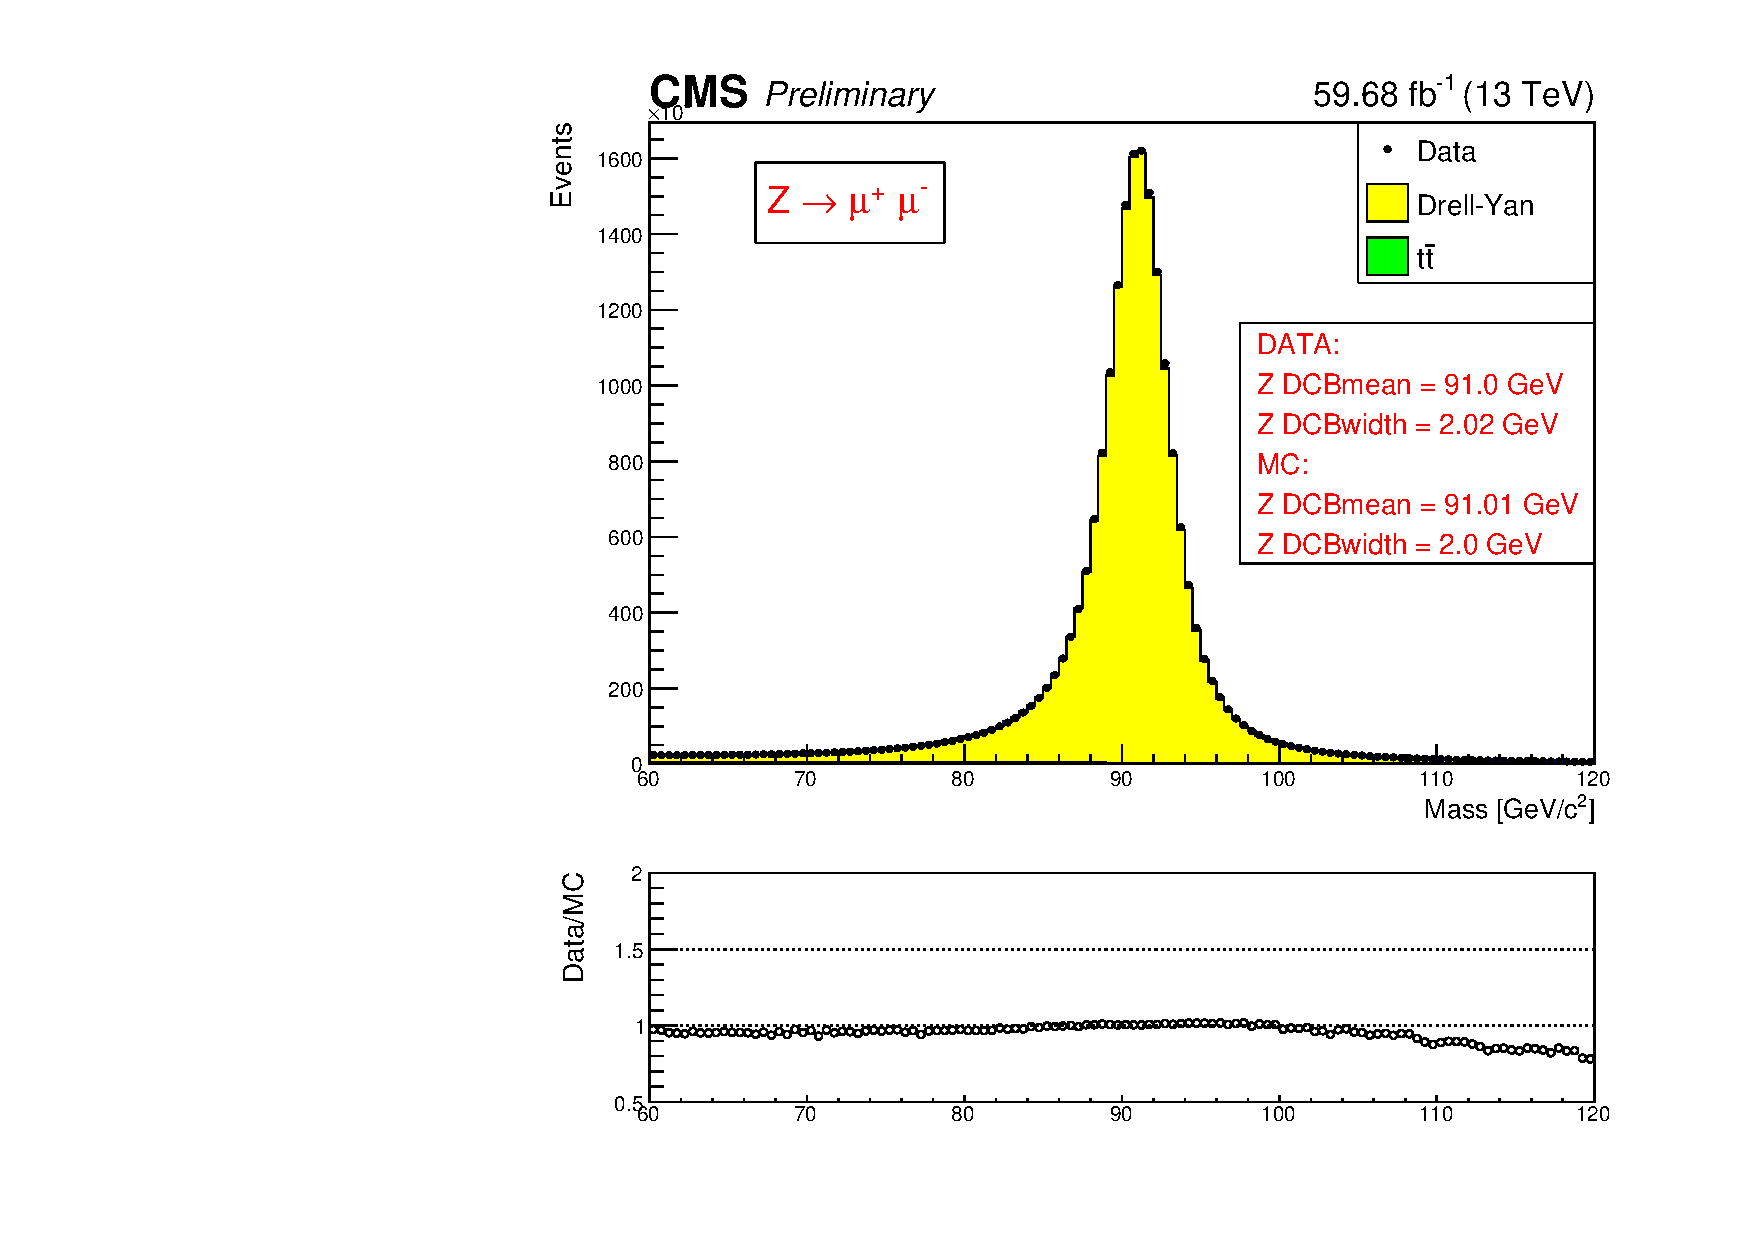
\includegraphics{Figures/Muons/2018_ZMass_mu_MBME.pdf}}}
%		\subfigure [] {\resizebox{8cm}{!}{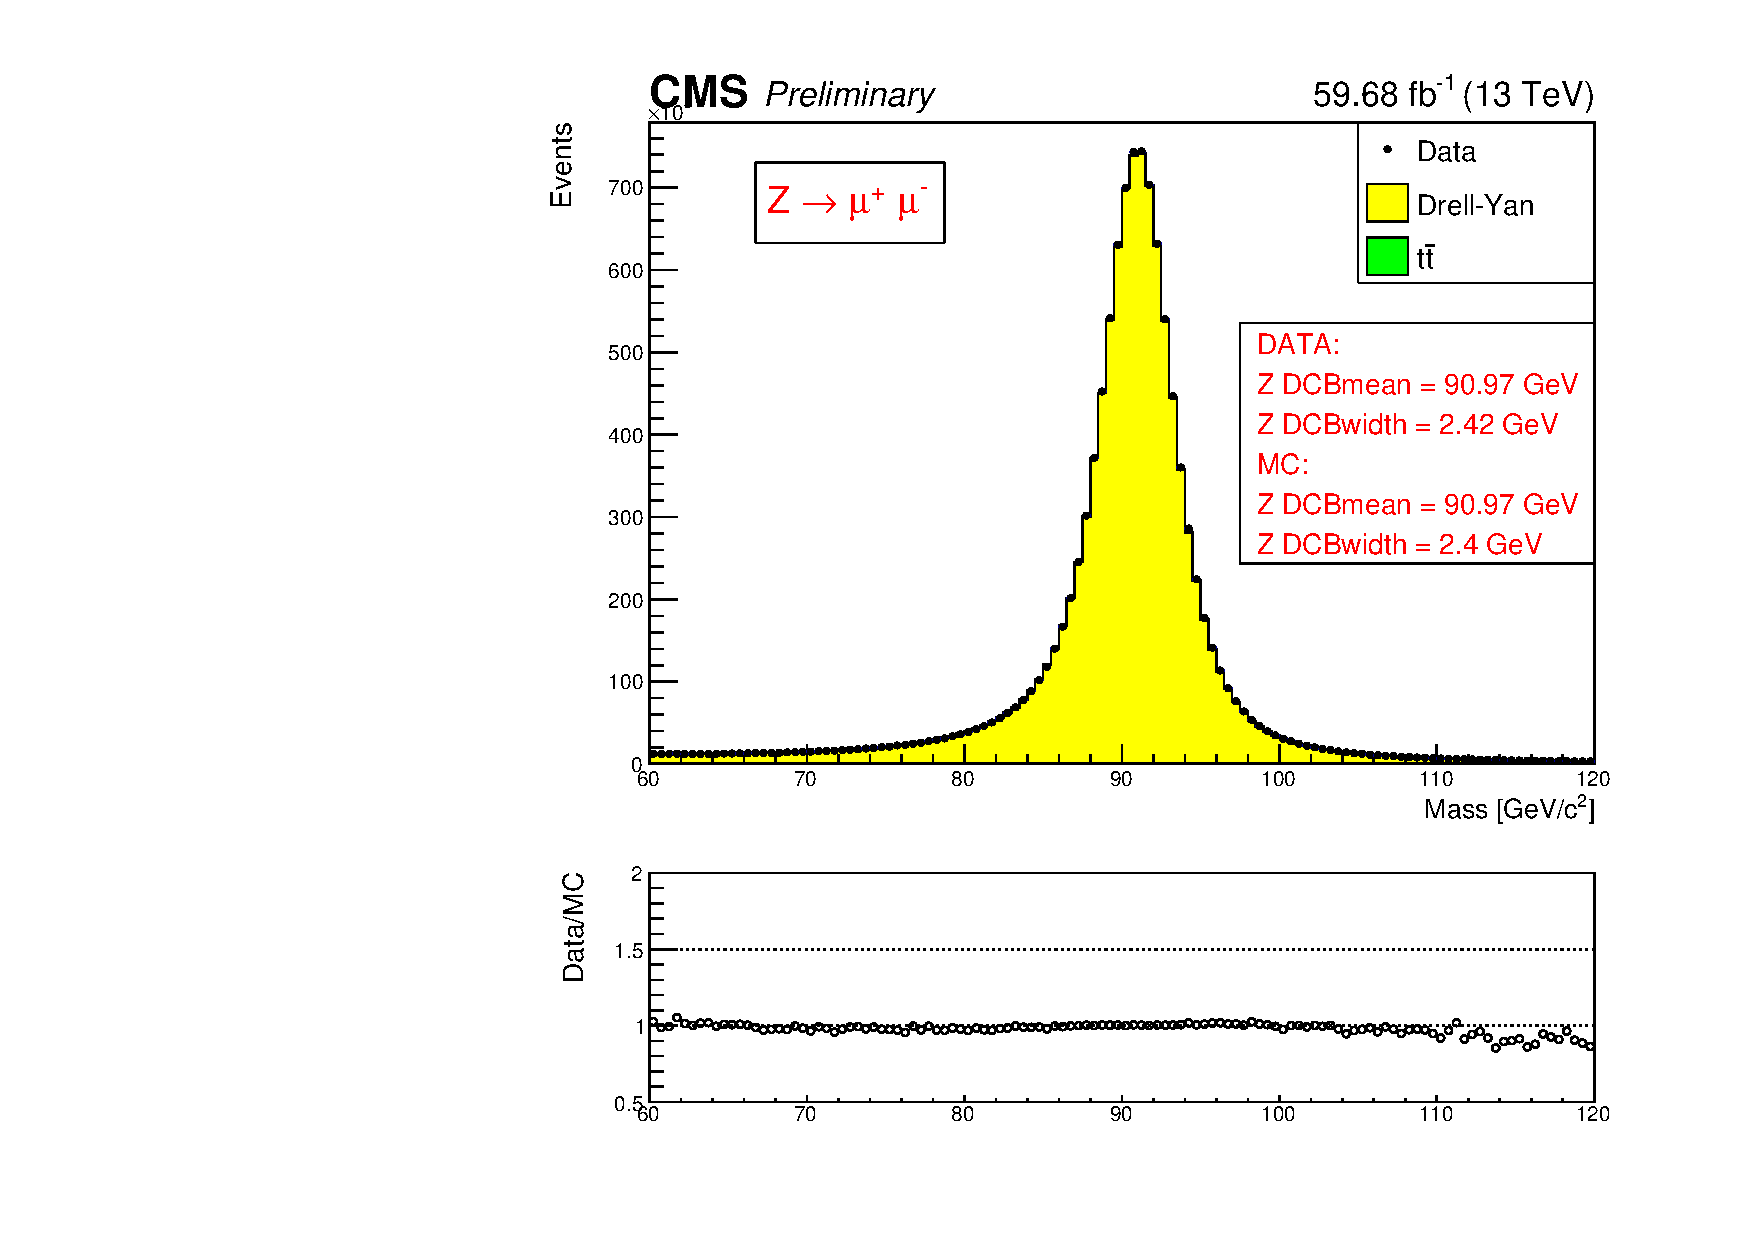
\includegraphics{Figures/Muons/2018_ZMass_mu_MEME.pdf}}} \\
%	\end{center}
%	\caption{
%		(a): muon energy scale measured in the $Z\rightarrow \mu \mu$ control region for all muons, for both muons in the barrel (b), for one muon in the barrel, one in the endcaps (c) and for both muons in the endcaps (d), for 2018.
%		The results of the Crystall-ball fit are reported in the figures.
%		%\textbf{FIXME: mu-scale and smearing corrections NOT yet available and thus NOT yet applied} 
%	}
%	\label{fig:mu_energy_scaleC}
%\end{figure}
%
%\clearpage
